\documentclass[a4paper, 11pt]{article}

%%% Zeichenkodierung, Rechtschreibung und Umlaute
\usepackage[utf8]{inputenc}
\usepackage[ngerman]{babel}
\usepackage[T1]{fontenc}

%%% Mathematische Symbole, Gleichungen
\usepackage[fleqn]{amsmath}
\usepackage{amsfonts}
\usepackage{amssymb}
\usepackage{amsthm}
\usepackage{mathtools}
\usepackage{bm}
%\usepackage{colonequals} % Zusätzliche Relationssymbole

%%% Tabellen
\usepackage{tabularx}
\usepackage{array}
\usepackage{multicol}
\usepackage{float}

%%% Seitenformat und -ränder
%%% -Alternative 1-
\usepackage{geometry}
\geometry{a4paper, top=25mm, bottom=20mm, left=20mm, right=20mm}
%%% -Alternative 2-
%\usepackage[headheight=110pt]{geometry}
%\geometry{a4paper,left=30mm,right=30mm, top=35mm, bottom=30mm}

%%% Seitenstile (Kopf- und Fußzeile)
\usepackage{fancyhdr}
\pagestyle{fancy}

%%% Sonstiges
\usepackage{caption} % Untertitel von Grafiken/Tabellen manipulieren
\usepackage{enumerate} % Aufzählungszeichen ändern
\usepackage{graphicx} % Standarderweiterung für Bilddateien
\usepackage{hyperref} % Hyperlinks
\usepackage{lastpage} % Berechnung der Seitenzahl
\usepackage{polynom} % Polynomdivision
\usepackage{setspace} % Zeilenabstand
%\usepackage{textgreek} % griechische Symbole
\usepackage{tikz} % Umfassendes Tool, um Grafiken zu erstellen
\usepackage{verbatim} % Schreibmaschinen-Stil (für Code-Ausschnitte)
\usepackage{float}

%%% Eingaben (z.B. für das Deckblatt)
\newcommand{\moduleabrv}{EDS Gruppe 15}
\newcommand{\module}{Embedded System Design Protokoll}
\newcommand{\semester}{Beuth Hochschule - Sommersemester 2018}
\newcommand{\finishingdate}{02.10.2018}
\newcommand{\titletextabrv}{       A/V Streaming}
\newcommand{\titletext}{Audio Video Streaming}

%%%-- Für das Deckblatt --
\title{
	~\\[4cm]
	\textbf{
		\module\\[0.25cm]
		\normalsize \semester \\[1.5cm]
		\Huge\titletext\\
	}
}

\author{
  \vspace{3.5cm}\\
  \begin{tabular}{l}
    \textbf{Gruppe 15:}\\\hline
    Omid Rahimian Mashhadi Mat.Nr.: 872958\\
    Torsten Michael Schenk Mat.Nr.: 838995\\
  \end{tabular}
}

\date{
	\vfill
	Abgabedatum: \finishingdate\\
	\vspace{5mm}
	Seitenanzahl: \pageref{LastPage}
}

%%% -- Kopf- und Fußzeile --
%%% Kopfzeile linker Bereich
\lhead[\leftmark]{\textbf{\moduleabrv}}
%%% Kopfzeile mittlerer Bereich
\rhead[\rightmark]{\rightmark{\titletextabrv}}
%%% Kopfzeile linker Bereich
%%\rhead{\textbf{zum \finishingdate}}
%%% Fußzeile
\cfoot{\thepage  \ / \pageref{LastPage}}

%%% Serifenfreie Fonts benutzen
%\renewcommand{\familydefault}{\sfdefault}

%%% Font
\usepackage{charter}

%%% Tiefe der Einrückung nach Absätzen
\setlength{\parindent}{0pt}

%%% Evtl. Änderungen des Typs einer Aufzählungsebene (z.B. zur Anpassung an das Aufgabenblatt)
%\renewcommand{\labelenumi}{\alph{enumi})}
%\renewcommand{\labelenumii}{(\roman{enumii})}
%\renewcommand{\labelenumiii}{\arabic{enumiii}.}
%\renewcommand{\labelenumii}{\textbf{-}}

\begin{document}

%%% Deckblatt
\maketitle
\thispagestyle{empty} % Keine Seitenzahl hier

\newpage
%\renewcommand\contentsname{Inhalt}
%\tableofcontents
    {\pagestyle{plain}
    \tableofcontents
    \cleardoublepage
    }

%\newpage
%%% Seitenzahl zurücksetzen
%\clearpage
%\setcounter{page}{1}

%%% Zeilenabstand
%\singlespacing
\onehalfspacing
%\doublespacing

%%%-- Eigentlicher Inhalt --
\section{Vorwort}
Für den Support und Bereitstellung von Hardware bedanken wir uns herzlich bei Herrn Krinke von der pi4\_robotics GmbH Berlin und für die beratende Funktion danken wir den Dozenten und Professoren der Beuth Hochschule Prof. Löwis, Dr. Flemming und Prof. Görlich.\\
Bei der Recherche zur Bearbeitung des Projektes wurden viele englische Webseiten zu rate gezogen und auch die man-pages der meisten Programme sind in Englisch verfasst. Generell kann man sagen, dass englische Fachbegriffe sich im Bereich Software etabliert haben, so dass eine Übersetzung eher verwirren als helfen würde. Daher haben wir uns entschieden, die \textbf{englischen} Bezeichner und Beschreibungen von Flags und Optionen beizubehalten.\\
Um Codeabschnitte besser von Beschreibungen unterscheiden zu können, wurde eine eigene Schriftart verwendet:
\begin{verbatim}
  Kommandozeilen Eingaben und Codesnippets werden wie HIER dargestellt.
\end{verbatim}

\section{Projektbeschreibung}
Das erklärte Ziel der pi4\_robotics GmbH Berlin ist es humanoide Roboter weiter zu entwickeln. 
Diese können bereits in unterschiedlichen Branchen eingesetzt werden. Im Werbeblatt 
des Workerbot4 (siehe Anhang, Kapitel \ref{RefAnhang}) werden die Basisfähigkeiten des Jolandi Workerbot beschrieben.  \\
Bisher ist das Anlernen neuer Tätigkeiten und die Bedienung nur über eine PC-Schnittstelle möglich. Doch das soll sich ändern. Geplant ist Spracherkennung und visuelle Wahrnehmung 
zu integrieren, um mit dem Roboter wie mit einem Menschen kommunizieren zu können. Auch soll 
ein Avatar Modus implementiert werden, bei dem der User in die Rolle des Roboters schlüpft 
und per Teleoperation den Roboter bewegt, hört was der Roboter hört und mit den Augen des Roboters sieht. \\
\begin{minipage}{\textwidth}
    \begin{center}
        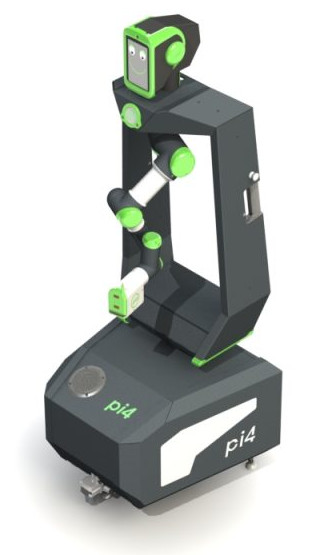
\includegraphics[scale=0.5]{img/jolandi.jpg} 
    \end{center}
\end{minipage}
\begin{center}
Jolandi Workerbot der Firma pi4\_robotics GmbH
\end{center}
 
\begin{minipage}{\textwidth}
    \begin{center}        
        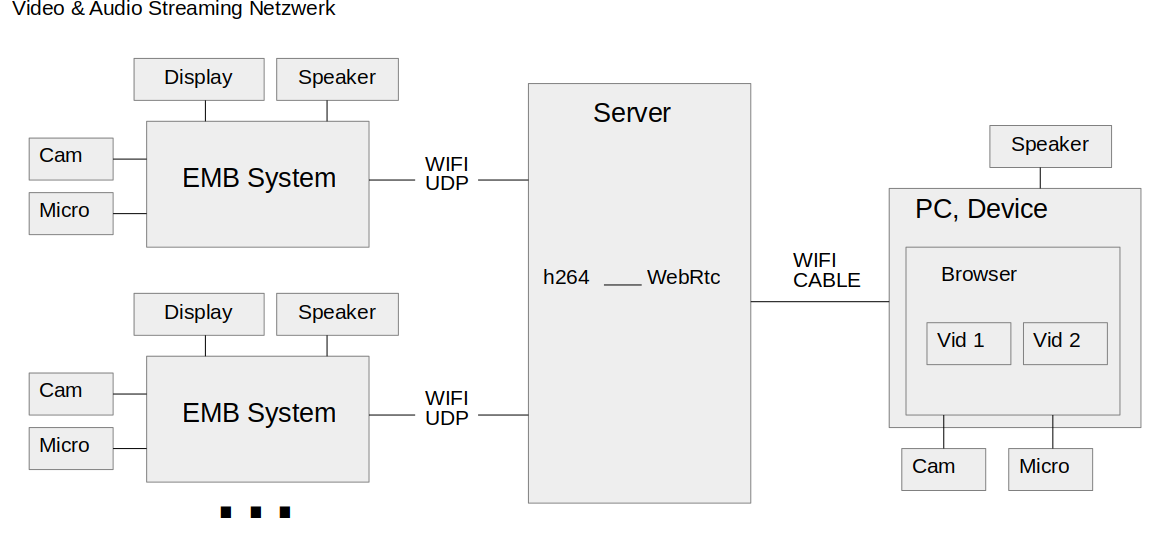
\includegraphics[scale=0.4]{img/schemaproj.png} 
    \end{center}
\end{minipage}
\begin{center}
Schemaplan der Komponenten
\end{center}
Für den Einsatz als Sicherheitspersonal ist weiterhin geplant, die Stimme des Bedieners aus dem Roboter Lautsprecher ertönen zu lassen und sein Gesicht auf dem Kopfdisplay anzuzeigen. 
Der Kunde soll das Gefühl haben, dass der Roboter der Avatar des Bedieners ist.\\
Für die Laborübungen 'Entwurf eingebetteter Systeme' und 'Netzwerk-Programmierung' wurde 
bidirektionale Ton und Video Übertragung ausgewählt. Dabei galt es Audio und Video \textbf{mehrerer} Roboter auf eine Webseite zu streamen und eine Webcam inklusive Ton des PC auf alle verbundenen Roboter zurück zu streamen.\\

Der Schemaplan zeigt den grundlegenden Aufbau des Komplettsystems. Auf der linken Seite sind 'n' integrierte eingebettete Systeme gezeigt, wie sie in pi4\_robotics GmbH Robotern verbaut sind. Pro Roboterkopf ist ein Raspberry PI mit Touch-Display vorhanden. Für das Projekt wurde jeweils eine Webcam für Ton und Video angeschlossen. Die Tonwiedergabe erfolgt über einen USB Lautsprecher. Die Anzeige des empfangenen Videostreams soll \textbf{ohne} Webbrowser erfolgen.\\
Auf der rechten Seite des Plans ist der Bediener PC dargestellt. Auch hier liefert eine Webcam Ton und Video. Der empfangene Audiostream wird über die PC Lautsprecher ausgegeben.\\
Für den Bediener soll ein \textbf{Web-Template} erstellt werden. Dort kann dieser auswählen, welcher Videostream angezeigt werden soll. Der Zeitversatz bei der Übertragung soll sehr gering sein 
(<0.2sek), damit der User möglichst schnell reagieren kann. Bildübertragung zum eingebetteten System darf einen leichten Zeitversatz haben, da dort nur das Gesicht des Bedieners angezeigt wird, aber keine weiteren Handlungen davon abhängen.\\
Das gesamte Streaming soll über das Internet erfolgen. Dabei ist der Datentransfer auch aus 
fremden WLAN Netzen heraus zu realisieren. Fremd im Sinne, dass die dazwischen liegenden Router und Ports nicht konfiguriert werden können. Die IP Adressen der Roboter sind damit quasi unbekannt, d.h. dynamisch wechselnd oder/und nicht vom Internet aus sichtbar, d.h. es ist nicht möglich direkt vom Sender zum Empfänger zu streamen.\\
Eine weitere Anforderung war, den Datentransport möglichst Effizient zu gestalten. Für den Upload ins Internet sollte ein Transportprotokoll mit geringem Overhead gewählt werden und für das Streaming auf die Webseite ein natives Format, welches von aktuellen Browsern unterstützt wird. Die Visualisierung sollte in Html5 \& Javascript ohne Browser-Plugins, Flash o.ä. erfolgen. Für die Realisierung musste also eine Möglichkeit gefunden werden, das Upload Format zu konvertieren und die Webseite mit einem Audio- und Videostream zu versorgen. Eine Streaminglösung über das Web erfordert drei Basiskomponenten um die Aufgabe zu erfüllen. Einen Streaming Server, einen Sender und einen Empfänger.

\textbf{Streaming-Server:} 
Ist die Hauptkomponente, die Audio- und Videoinhalte von den Sendern an die Empfänger weiterleitet. Gleichzeitig kann auch die Konvertierung von einem Format oder Codec in ein anderes erfolgen.

\textbf{Sender:} Eine Quelle, die einen Audio- und Videostream zum Server schickt. 

\textbf{Empfänger:} Ein Empfänger, der sich mit dem Stream vom Server verbindet und diesen abspielt oder speichert.
\section{Realisation} \label{RefIntro}
Schon bei Projektstart wurde klar, dass es sich um sehr umfangreiche Anforderungen handelt. Es galt nicht nur eine Streaming Lösung zu implementieren, sondern es mussten auch alle Hardwarekomponenten getestet und angesteuert werden. Für die Bedienerseite musste eine funktionale Webseite einschließlich Webserver erstellt werden und ein Streaming-Server für die Konvertierung und Vernetzung der Sender und Empfänger musste konfiguriert werden. Viele \textbf{wichtige} bisher nicht genannte Anforderungen, z.B. Cybersicherheit, Authentifizierung wurden weitestgehend außer acht gelassen. Sie sind natürlich für eine endgültige industrielle Anwendung unerlässlich.\\

Das Projekt wurde in Teil-Aufgaben realisiert:
\begin{itemize}
\item Inbetriebnahme aller Hardwarekomponenten

\item Direktes Streamen von Audio und Video vom embedded System an PC
\item Aufsetzen eines Streaming-Servers im lokalen Netzwerk
\item Aufsetzen eines Webservers im lokalen Netzwerk, lokales hosting der Webseite
\item Direktes Streamen von Audio und Video vom embedded System an Streaming-Server
\item Anzeige des konvertierten Outputs des Streaming-Servers auf der Webseite
\item Streamen der PC Webcam an lokalen Streaming-Server
\item Zurück-Streamen vom Streaming-Server an embedded Hardware und Visualisierung
\item Hochladen der Webseite auf eine Online-Webspace
\item Aufsetzen eines Online-Streaming-Servers
\end{itemize}

\subsection{Inbetriebnahme der Hardware Komponenten}
Am Anfang des Projektes wurden alle Hardwarekomponenten bestellt und getestet. Raspberry PI B3+, Touchdisplays, Gehäuse, USB Lautsprecher, Webkameras mit Mikrofon und MMC Karten, siehe Lastenheft auf www.trello.com (Gruppe 15) für eine detaillierte Hardwareaufstellung. Danach kam die Installation des Betriebssystems RASPIAN auf den Raspberry PI3+ Boards und die Konfiguration eines Zugangs über SSH, siehe Kapitel \ref{RefRaspi}. Kleine Nebenarbeiten waren das softwareseitige Drehen des Displays und Touchdisplays, sowie das Upgraden und Updaten der vorinstallierten Pakete.\\
Für Audio und Video Tests wurden *.mp4 Files und *.wav Dateien abgespielt, siehe Kapitel \ref{RefLautsprecher}. WLAN befindet sich bereits bei PI3+ als Komponente auf dem Board und musste nur konfiguriert werden. Die Mikrofon Tests gestalteten sich anspruchsvoller und es wurden Facebook Chat und WebRTC Internet Beispiele verwendet.

\subsection{Streaming: embedded System > Server > Webseite}
Um A/V Streaming auf dem Raspberry zu starten, wurden ffmpeg und gstreamer mit den 
vorkompilierten Paketen über den Paketmanager installiert. Wobei gstreamer den vollen Funktionsumfang (verglichen mit Ubuntu 18) hatte. Für Installationsanleitung und kompletter Liste der Testbefehle zu gstreamer, siehe Kapitel \ref{RefGstreamer}. \\
Die Verwendung von ffmpeg gestaltete sich jedoch problematisch. Die Pakete des Paketmanagers unterstützten weder ffserver noch ffplay und es fehlten Abhängigkeiten zu diversen Bibliotheken. Es war nötig ffmpeg aus den Quellen zu bauen, siehe Kapitel \ref{RefFFmpeg} mit Schritt für Schritt Anleitung und alle durchgeführten Tests. Bei der Installation stellte sich heraus, dass ffserver nicht mehr in der aktuellen Version 4 unterstützt wird und es wurde via Git die Version 3.4 ausgecheckt. Dies bewirkte eine Kettenabhängigkeit der x264 Bibliothek, deren Version nun ebenfalls herunter gesetzt werden musste. Schließlich stand eine voll funktionsfähige ffmpeg, ffserver und ffplay Version bereit.\\ 

\textbf{Direktes A/V Streamen vom embedded System > PC}\\
Versuche mit ffmpeg A/V Streaming wiesen ein Delay von >2.5s zwischen senden und empfangen auf. Die Testergebnisse sind in Tabelle \ref{tbl:beispieltabelle} Kapitel \ref{RefVergleich} zusammengefasst. Der Stream wurde mit ffmpeg erzeugt und an den ffserver auf dem PC geschickt. Das Ergebnis \textbf{(m)} in Tabelle \ref{tbl:beispieltabelle} stellte das KO Kriterium dar. 2.5 Sekunden waren zuviel, um einen interaktiven Chat zu gestalten. PC seitig konnte daran nichts geändert werden. ffplay, mplayer und vlc wurden ohne Verbesserung des Ergebnisses getestet.\\
Gstreamer konnte dieses Ergebnis bei weitem übertreffen. A/V Streaming ohne Server war nahezu ohne Verzögerung ca. 0.1s, siehe Testergebnis \textbf{(h)} in Tabelle \ref{tbl:beispieltabelle}, Kapitel \ref{RefVergleich}. Gstreamer erfüllte damit die Anforderung und wurde im weiteren Projekt verwendet, um A/V direkt an den Streaming-Server zu senden.\\

\textbf{Aufsetzen eines Streaming-Servers im lokalen Netzwerk}\\
Die Auswahl eines OpenSoure Streaming Servers gestaltete sich schwierig. Die Anforderung einen A/V Stream möglichst Overhead frei, z.B. RTP/UDP Format, in ein Web natives Format zu konvertieren erforderte viel Recherchezeit. Dazu kommt noch, dass veröffentlichte Projekte meistens nicht passend sind und z.B. auf Browser zu Browser Streaming basieren. Alternativ handelt es sich um Streaming-Lösungen, die ganz ohne Browser arbeiten. Die gesetzte Anforderung aus einem eigenen Programm ohne Browser auf eine Webseite zu streamen und wieder zurück, erschwerte den Fortschritt des Projektes. Dazu kam noch, dass zwar Video Streaming generell gut dokumentiert ist, aber in Kombination mit Audio nicht häufig Verwendung findet. Das liegt hauptsächlich daran, dass die meist verkaufte RASPI-CAM kein Mikrofon besitzt und deshalb fast alle Tutorials und Dokumentationen nur Video Streaming beschreiben. Viele Start-Ups werben mit Lösungen, welche die A/V Anforderung im Projekt erfüllen würden. Es scheint ein Bereich unter aktiver Entwicklung zu sein, wie von und zu embedded Systemen A/V gestreamt werden kann.\\
Schließlich wurden UV4L und das Janus-Gateway in die engere Auswahl gezogen. Die UV4L Bibliothek erwähnt zwar eine Einsatzmöglichkeit auch ohne Webbrowser auf den Klientseite. Es konnte jedoch keine ausreichende Dokumentation gefunden werden, wie UV4L zum direkten A/V Streaming verwendet wird. Beim Janus-Gateway stand zumindest eine Standard-Konfiguration für RTP zu WebRTC bereit und in Foren werden Probleme nicht korrekter Konfiguration diskutiert. Auch ist das Empfangen von gstreamer RTP-Paketen möglich. Die Installation und Konfiguration des Janus-Gateways ist in Kapitel \ref{RefJanus} beschrieben. Das Janus-Gateway wurde im weiteren Projektverlauf verwendet, um mehrere RTP Streams von embedded Systemen zu empfangen und als WebRTC Streams via http auf eine Webseite weiterzuleiten.\\

\textbf{Aufsetzen eines Webservers im lokalen Netzwerk, Hosting der Webseite}\\
Als Webserver wurde nginx ausgewählt, um eine Webseite im lokalen Netzwerk zu hosten. Die Demo-Webseiten des Streaming-Servers benötigen noch diverse Anpassungen, um z.B. den Admin/Monitor verwenden zu können. Erst danach steht mit nginx eine vollwertige Entwicklungsumgebung zur Verfügung. Installation und Konfiguration von nginx wird in Kapitel \ref{Refnginx} erklärt.\\

\textbf{Direktes Streaming von Audio und Video vom embedded System an den Streaming-Server}\\
Gstreamer Befehle für die Übertragung von A/V vom Raspberry an das Janus-Gateway sind in Kapitel \ref{RefGstrToJanus} aufgelistet.

\subsection{Webseite zur Anzeige der Videostreams}
Die Janus-Installation enthält bereits Demowebseiten für die Anzeige der WebRTC Streams und Werkzeuge für die Konfiguration von Chaträumen. Mittels einer Debug Admin/Monitor Seite können eingehende Streams, Anzahl der Pakete, IP-Adressen usw. angezeigt werden. Der bereit gestellte Javascript-Code kann verwendet werden, um interaktiv Kamera und Mikrofon des Bedieners auszuwählen. Im Rahmen des Projektes wurde durch Änderung der Demowebseiten eine funktionale Testwebpage gestaltet, um wahlweise die A/V Streams verschiedener emb.Systeme anzeigen zu können.\\

\begin{minipage}{\textwidth}
    \begin{center}
        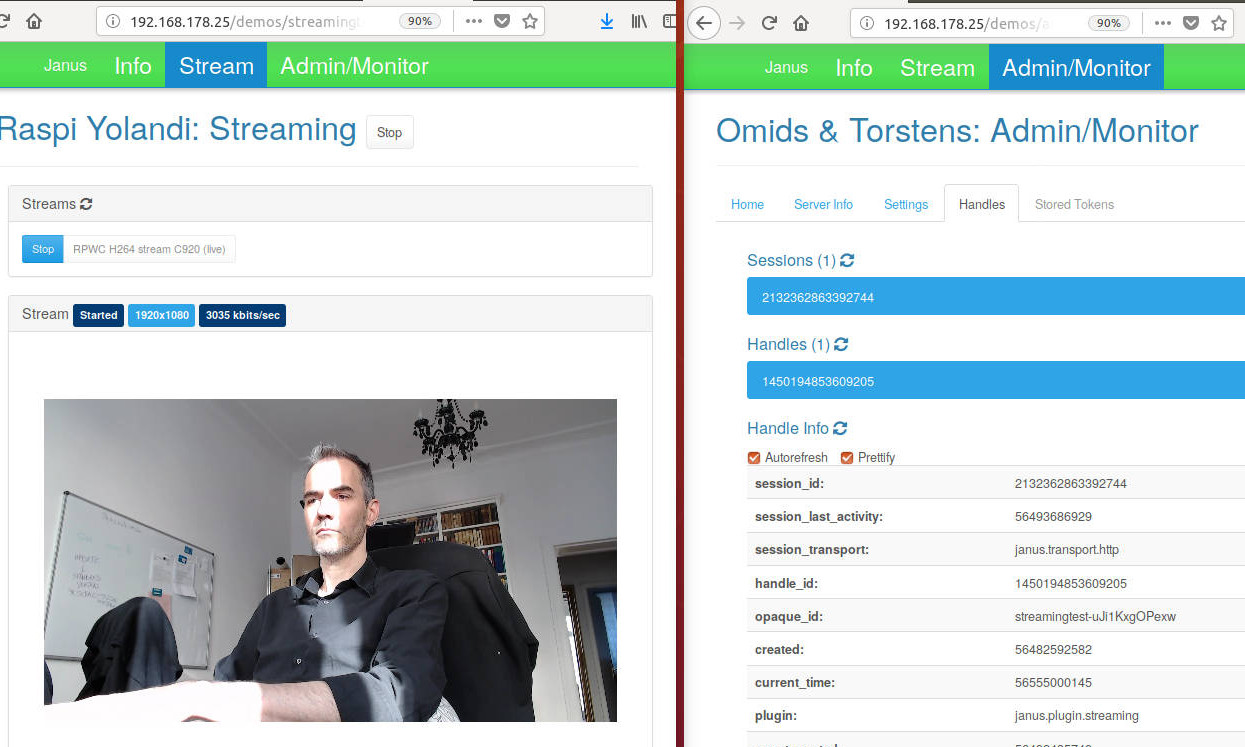
\includegraphics[scale=0.27]{img/janusweb.jpg} 
    \end{center}
\end{minipage}
\begin{center}
Adaptierte Website zur Anzeige der A/V WebRTC-Streams
\end{center}

\subsection{Streaming: PC > Server > Anzeige auf embedded System}
Wie der Test \textbf{(i)} in Tabelle \ref{tbl:beispieltabelle} Kapitel \ref{RefVergleich} gezeigt hat, ist gstreamer ungeeignet, um A/V auf den Raspberry zurück zu streamen. Die Framerate konnte nicht festgestellt werden, da das Entpacken und Decodieren der Formate zu langsam ist. Die CPU Leistung ist nicht ausreichend. Es wurden VP8, h264 Komprimierung und auch raw getestet, jedoch ohne Erfolg.\\

Ffmpeg blieb mit dem Testergebnis \textbf{(n)} mit >1.5s Delay die einzige funktionale Lösung. Der ffserver wurde so konfiguriert, dass die eingehenden http Pakete zu webm konvertiert werden. Auf dem Raspberry werden diese nur noch zur Anzeige gebracht, ohne aufwändiges Dekodieren. In Kapitel \ref{RefBack} sind die Konfiguration und Kommandozeilen-Eingaben aufgelistet. Das WebM Format kann auch im Browser angezeigt werden. Auf dem Raspberry trat jedoch im Browser ein Delay von15s auf! Alle Versuche A/V auf den Raspberry zurück zustreamen resultierten in 100\% CPU Last. Die Bibliotheken verwenden zwar Hardwareunterstüzung beim Kodieren und Komprimieren der Videoframes, aber nicht beim Dekodieren. Es müsste noch untersucht werden, ob eine Hardwareunterstützung für beide Aufgaben gleichzeitig erfolgen kann und ob dies von den Bibliotheken unterstützt wird. Der Standard ist es, Video vom leistungsschwachen System mit Hardwareunterstützung zu verschicken.\\

\begin{minipage}{\textwidth}
    \begin{center}
        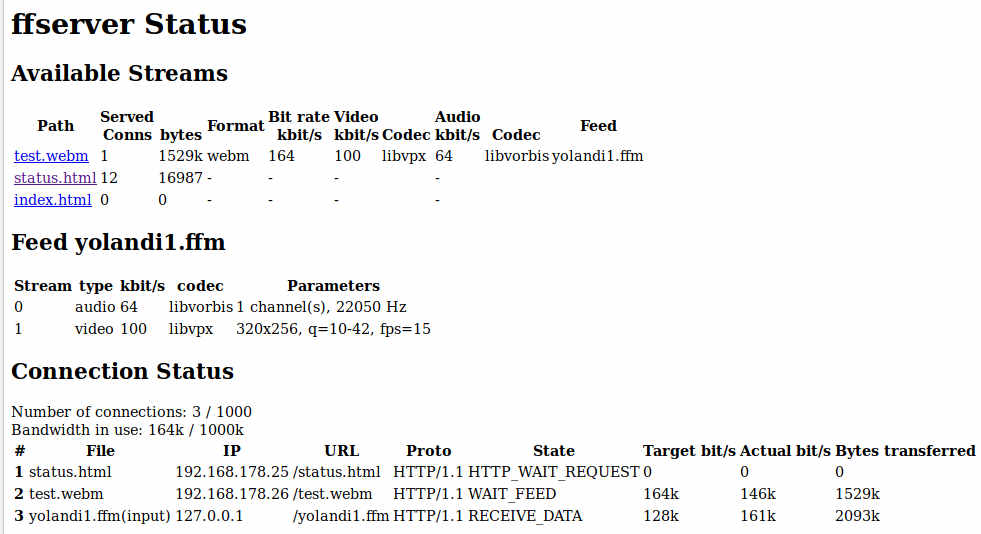
\includegraphics[scale=0.5]{img/statusff.jpg} 
    \end{center}
\end{minipage}
\begin{center}
Status ffserver Webpage zur Anzeige der verbundenen Streams
\end{center}

Der ffserver kann eine Status Webseite generieren, mit der fps, verbundene Klienten und eingehende Streams angezeigt werden können, siehe Screenshot.\\
Das zurück Streamen wurde für das Projekt mit ffmpeg auf PC Seite und ffserver auf dem Server realisiert. Der Raspberry Klient kann den webm http Stream direkt von der IP-Adresse und Port des Servers erhalten und via ffplay anzeigen. Als optionale Lösung könnte auch Audio getrennt von Video gesendet werden. Dann sollte Audio nahezu ohne Delay wiedergegeben werden können und Video mit ca. 1.5s Verzögerung.

\subsection{Online Setup}
Alle beschriebenen Tests und Installationen wurden auf PC und im lokalen Home-Netzwerk durchgeführt. Dies geschah mit dem Ausblick eine Lösung für das www zu entwickeln. Schließlich wurden gegen Ende es Projektes noch einige Tests im Internet durchgeführt. Dabei ging es um die Funktionalität der Webseite und die Ports des Streaming-Servers, leider konnten die Versuche noch nicht abgeschlossen werden.\\ 

\textbf{Hochladen der Webseite auf eine Online-Wespace}\\
Die angepasste Demo-Webseite wurde via Filezilla auf eine Strato-Webspace hochgeladen. Sie ist voll funktionsfähig und kann under \textit{www.witchplease.de} angezeigt werden. Der Janus-Webserver ist nicht durchgehend aktiv und wird nur zu Testzwecken gestartet. Wie schon am Anfang von Kapitel \ref{RefIntro} beschrieben wurde die Kommunikation noch \textbf{nicht} sicher gestaltet.\\

\textbf{Aufsetzen eines Online-Streaming-Servers}\\
Der Zugang zum Server erfolgte mit ssh und darauf aufbauend kann per VNC eine remote Desktopverbindung geöffnet werden. Eine Beschreibung ist in Kapitel \ref{RefStrato} zu finden. \\

\textbf{Webserver Verbindungstest}\\
Bei den gstreamer Versuchen wurde zuerst mit Wireshark untersucht, ob die RTP Pakete an den Ports der Servers ankommen. Der Screenshot zeigt den gstreamer Befehl und einen Ausschnitt der Wireshark gui.\\
Im oberen Bereich ist der gstreamer Befehl mit dem Audio udpsink host...5000 und Video udpsink...5001. Wireshark detektiert ankommende Pakete im Webserver (ip 85.214.211.169) vom raspberry pi (ip 77.14.37.230) an den UDP Ports 5000 (Audio Paketgröße 451) und UDP 5001 (Video Paketgröße 894).\\

\begin{minipage}{\textwidth}
    \begin{center}
        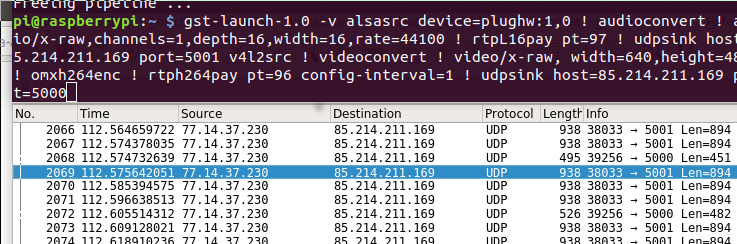
\includegraphics[scale=0.7]{img/wireshark.png} 
    \end{center}
\end{minipage}

\begin{center}
Wireshark detektiert ankommende Pakete an den Server-Ports
\end{center}

\subsection{Ergebnis}
Es konnte eine Streaming Lösung entwickelt werden, die A/V von mehreren Raspberry PiB3+ über WLAN auf eine Webseite streamt. Auf der Webseite kann ausgewählt werden, welcher Stream angezeigt werden soll. In einem Admin/Monitor können die verbundenen Streams mit umfangreichen Kenndaten ausgewertet werden. Im Detail sieht die Streaming Lösung wie folgt aus:
\begin{verbatim}
n * Raspi Webcam & Audio > gstreamer > RTP/UDP > Janus-Gateway > Http/WebRTC > Webseite
\end{verbatim}

Für das zurück Streamen, der am PC integrierten oder einer externen Webcam mit Audio, wurde ffmpeg und ffserver sowie ffplay verwendet. Dabei wird ein, mittels ffmpeg erzeugter Stream vom ffserver in das webm Format konvertiert und auf dem Raspberry mit ffplay ohne aufwändiges Dekodieren angezeigt. Im Detail sieht die zurück Streaming Lösung wie folgt aus:
\begin{verbatim}
PC Webcam & Audio > ffmepg > http > ffserver > http/webm > n * Raspi ffplay
\end{verbatim}

Die gesetzten Anforderungen konnten damit voll erfüllt werden. Es ist möglich von mehreren Raspberries auf eine Webseite zu streamen und die Webcam des Users auf alle verbundenen Raspberries zurück zu streamen. Auf dem Raspberry PI können alle Streams generiert und empfangen werden, ohne dass ein Webbrowser benötigt wird und verwendeten Bibliotheken ffmpeg und gstreamer können sogar auch direkt in eigene Programme integriert werden. Die Kommandozeilen-Befehle können z.B. auch direkt beim Systemstart aktiviert werden, so dass ein manuelles Aktivieren entfällt. Für den Bediener wurde eine einfach zu handhabende Webseite bereit gestellt, um die Streams anzuzeigen. \\
Zu allen verwendeten Werkzeugen wurden ausführliche Installationsanleitungen geschrieben und die Tests dokumentiert.\\

\textbf{Ausblick}\\
Ideal wäre das zurück Streamen auch über WebRTC zu realisieren. Die Javascript Bibliotheken sind verfügbar und ermöglichen dem User das Auswählen der gewünschten Kamera und des Mikrofons auf dem eigenen PC. UV4L könnte den Empfang des WebRTC Streams auf dem Raspberry PI ohne Browser realisieren.

\section{Software Helfer}
Kurze Beschreibung der Software Hilfsprogramme

\subsection{Paket Manager}
Pakete des Raspian Betriebssystems auf neustem Stand halten
\begin{verbatim}
  sudo apt update
  sudo apt upgrade
  z.B. Firefox für Raspi installieren: sudo apt install firefox-esr
\end{verbatim}

\subsection{Video Formate der Kamera}
Vor Auswahl eines Bildformates alle unterstützten Formate abfragen:
\begin{verbatim}
  v4l2-ctl --list-formats-ext
\end{verbatim}

oder über USB Gerätekennung und danach all Höhen und Breiten abfragen.
\begin{verbatim}
  lsusb
  > Bus 001 Device 016: ID 046d:082d Logitech, Inc. HD Pro Webcam C920
  > ...
  lsusb -s 001:016 -v | egrep "Width|Height"
\end{verbatim}

\textbf{Achtung:} Wenn ein nicht unterstütztes Video Format angegeben wird, bricht gstreamer mit nicht definiertem Fehler ab.
\begin{verbatim}
  v4l2src0: Internal data stream error.
\end{verbatim}


%%%%%%%%%%%%%%%%%%%%%%%%%%%%%%%%%%%%%%%%%%%%%%%%%%%%%%%%%%%%%%%%%%%%%%%%%%%
\begin{comment}
\section{Motion Installation \& Test}

Motion ist ein Programm, das in der Lage ist zu erkennen, wenn ein signifikanter Teil des Kamerabildes sich verändert. Es kann also Bewegung erkennen und einen Warnton übertragen. Es ist ein Kamera Streaming Service, welches verwendet werden kann, um den Videostream einer Webcam an eine IP Adresse zu leiten. Motion kann mit vielen Geräten verwendet werden. Unterstützt werden: V4L2 Webcams (closed source), Video Frame Grabber, Network Kameras via HTTP, RTSP, RTMP, PI Kameramodul, Webcam. Die Installationsanleitung für den Motion Streaming Server auf Raspian Betriebssystem folgt dem Tutorial auf \textit{https://pimylifeup.com/raspberry-pi-webcam-server/} und wurde um eigene Anpassungen erweitert.\\

\textbf{Raspian Version pi\_strech\_motion}

\begin{enumerate}
	\item Installation:
	\begin{verbatim}
	sudo apt-get install libmariadbclient18 libpq5 libavcodec57  libavformat57
	    libavutil55 libswscale4
	\end{verbatim}
	Einige Pakete sind veraltet und müssen durch aktuelle ersetzt werden:
	\begin{verbatim}	
	sudo apt install libx264-148 libavcodec57 libavformat57 libmariadbclient-dev-compat 	
	    default-libmysqlclient-dev libswscale
	\end{verbatim}
	\item Motion-stretch Debian Paket herunterladen
	\begin{verbatim}
	sudo wget https://github.com/Motion-Project/motion/releases/download/ \
	release-4.0.1/pi_stretch_motion_4.0.1-1_armhf.deb
	sudo dpkg -i pi_stretch_motion_4.0.1-1_armhf.deb
	\end{verbatim}
	\item Motion konfigurieren
	\begin{verbatim}	
	sudo vim /etc/motion/motion.conf
	daemon on
	stream_localhost off
	if problems with freezing if motion occures
	output_pictures off
	ffmpeg_output_movies off
	optional
	stream_maxrate 100
	framerate 100
	width 640
	height 480

	sudo vim /etc/default/motion
	start_motion_daemon=yes
	\end{verbatim}
\end{enumerate}

\textbf{Start \& Stopp Motion und Streaming}
\begin{verbatim}
sudo service motion start
sudo service motion stop
\end{verbatim}
Browser zur Anzeige im lokalen Netzwerk (Ip Adresse des Raspberry)\\
192.168.1.xxx:8081
\end{comment}
%%%%%%%%%%%%%%%%%%%%%%%%%%%%%%%%%%%%%%%%%%%%%%%%%%%%%%%%%%%%%%%%%%%%%%%%%
\section{ffmpeg, ffserver, ffplay} \label{RefFFmpeg}
\textbf{ffmpeg mit alsa auf Raspberry}\\
Die ffmpeg Pakete für (arm-hf), die über den Paketmanager installiert werden können, sind ohne \textbf{alsa} Abhängigkeit kompiliert worden. ffmpeg verwendet zum Audiostreaming jedoch häufig alsa. Bei Verwendung einer RASPI-cam wird alsa nicht benötigt, so dass die alsa Unterstützung bei den meisten Anwendung nicht benötigt wird. Für das Streaming Projekt musste deshalb ffmpeg aus den Quellen kompiliert werden. Die Version von ffmpeg 4 musste auf 3.4 herunter gesetzt werden, da ffplay und ffserver in Version 4 nicht mehr enthalten sind. ffserver und ffplay sind ideal, um im lokalen Netzwerk Streaming Pipelines zu testen. ffserver ermöglicht es eine Status html Webseite zu generieren, die fps, verbundene Klienten und vieles mehr anzeigt.\\ 

\textbf{Installation von FFmpeg aus Source-Code}
Wichtige Info: ffserver wurde beim Upgrade auf ffmpeg Version 4.0 gelöscht. Letzte Version mit ffserver ist 3.4. Daher git checkout 3.4! Wenn ffplay mitkompiliert werden soll muss zuerst sdl installiert werden:
\begin{verbatim}
  sudo apt install libsdl2-dev libsdl2-image-dev libsdl2-ttf-dev \
  libsdl2-mixer-dev
\end{verbatim}

Für libmp3lame > 3.88 bitte zusätzlich installieren:
\begin{verbatim}
  sudo apt install libmp3lame-dev
\end{verbatim}

Siehe auch:\\
http://computingvoyage.com/2114/installing-sdl2-on-raspbian-jessie/
\begin{verbatim}
#!/bin/bash
# ffmpeg install script by Schenk/Omid
# To make executable: chmod +x install.sh
# To install ffserver, you have to check out the 3.5 of 3.4 version of ffmepg git 
# repo to be able to compile ffmpeg with x264, you also have to choose an old 
# version from git repo tested was the version, before x264_bit_depth was removed 
# (needed for ffmpeg 3.4, 3.5)
# x264 hash key checkout: 7839a9e1f03b49e3e0cbfcb3091093af7c6d54ee
#
wget http://downloads.xiph.org/releases/vorbis/libvorbis-1.3.3.tar.gz
tar -xf libvorbis-1.3.3.tar.gz
cd libvorbis-1.3.3/
./configure --host=arm-unknown-linux-gnueabi --enable-static
make
sudo make install
cd ..
# libogg
wget http://downloads.xiph.org/releases/ogg/libogg-1.3.1.tar.gz
tar -xf libogg-1.3.1.tar.gz
cd libogg-1.3.1/
./configure --host=arm-unknown-linux-gnueabi --enable-static
make
sudo make install
cd ..
# libtheora
wget http://downloads.xiph.org/releases/theora/libtheora-1.1.1.tar.bz2
tar -xf libtheora-1.1.1.tar.bz2
cd libtheora-1.1.1/
./configure --host=arm-unknown-linux-gnueabi --enable-static
make
sudo make install
cd ..
git clone http://git.videolan.org/git/x264.git
cd x264
./configure --host=arm-unknown-linux-gnueabi --enable-static --disable-opencl
echo "Compiling x264"
make
sudo make install
cd ..
# extra alsa
wget ftp://ftp.alsa-project.org/pub/lib/alsa-lib-1.1.1.tar.bz2
tar xjf alsa-lib-1.1.1.tar.bz2
cd alsa-lib-1.1.1/
./configure --host=arm-unknown-linux-gnueabi --enable-static
make -j4
sudo make install
cd ..
# libvpx
git clone https://chromium.googlesource.com/webm/libvpx
cd libvpx
./configure --enable-static
make -j4
sudo make install
cd ..
# libsdl
wget http://www.libsdl.org/release/SDL-1.2.15.tar.gz
tar xzvf SDL-1.2.15.tar.gz
cd SDL-1.2.15
./configure --host=arm-unknown-linux-gnueabi --enable-static
make -j4
sudo make install
cd ..
git clone https://github.com/FFmpeg/FFmpeg.git
cd ffmpeg
./configure --arch=armel --target-os=linux --enable-gpl --enable-libx264 \
  --enable-nonfree --enable-libtheora --enable-libvorbis --enable-libvpx \
  --enable-libmp3lame
make
sudo make install
\end{verbatim}	
Hinweis: nachdem ./configure ausgeführt wurde, kann im Log kontrolliert werden, ob alle benötigten apps kompiliert werden. Es sollten die Bibliotheken, alsa, libx264, sdl2, libtheora, libxcb, libvpx und die Programme ffmpeg, ffserver und \textbf{ffplay} angezeigt werden.

\begin{verbatim}
External libraries:
alsa			libvorbis		libxcb_shape		sndio
iconv			libvpx			libxcb_xfixes		xlib
libmp3lame		libx264			sdl2			zlib
libtheora		libxcb

External libraries providing hardware acceleration:
v4l2_m2m

Libraries:
avcodec			avfilter		avutil			swresample
avdevice		avformat		postproc		swscale

Programs:
ffmpeg			ffplay			ffprobe			ffserver
\end{verbatim}

\subsection{ffmepg Optionen \& Flags}
Auswahl nicht Codec abhängiger Parameter mit moderner Schreibweise. Viele Tutorials enthalten das -an oder -av Flag zum temporären abschalten von Audio oder Video!
\begin{verbatim}
-formats   print the list of supported file formats
-codecs    print the list of supported codecs (E=encode,D=decode)
-i         set the input file. Multiple -i switchs can be used
-f         set video format (for the input if before of -i, for output otherwise)
-an        *** ignore audio
-vn        *** ignore video
-ar /-r    set audio rate (in Hz), -r also working
-ac        set the number of channels
-b:a /-ab  set audio bitrate
-b:v /-b   Video bitrate
-bt        Video bitrate tolerance
-c:a /-acodec  choose audio codec or use “copy” to bypass audio encoding
-c:v /-vcodec  choose video codec or use “copy” to bypass video encoding
-r         video fps. You can also use fractional values like 30000/1001 instead of 29.97
-s         frame size (w x h, ie: 320x240)
-aspect    set the aspect ratio i.e: 4:3 or 16:9
-sameq     ffmpeg tries to keep the visual quality of the input
-t N       encode only N seconds of video (you can use also the hh:mm:ss.ddd format)
-croptop, -cropleft, -cropright, -cropbottom   crop input video frame on each side
-y         automatic overwrite of the output file
-ss        select the starting time in the source file
-vol       change the volume of the audio
-g         Gop size (distance between keyframes)
-metadata  add a key=value metadata
\end{verbatim}

\subsection{ffmepg Tests}
Als erster Test kann ffmpeg dazu verwendet werden Videos mit oder ohne Audio zu speichern.\\
Dabei traten beim .ogg Format ungewöhnliche Speed-Ups oder Sprünge statt. Mp4 ist von 
ausgezeichneter Qualität. Der Befehl list\_formats zeigt alle von der Webcam unterstützten 
Formate an.\\

Die niedrigste Latenz kann mittels Flags für die Anzeige Apps erreicht werden:
\begin{verbatim}
  ffplay -fflags nobuffer 
  mplayer -benchmark
\end{verbatim}

Test nur Video:
\begin{verbatim}
  ffmpeg -f v4l2 -list_formats all -i /dev/video0

  ffmpeg -f v4l2 -r 25 -s 640x480 -i /dev/video0 out.avi
  ffmpeg -f v4l2 -r 25 -s 640x480 -i /dev/video0 out.mp4
  ffmpeg -f v4l2 -r 25 -s 640x480 -i /dev/video0 out.ogg
  ffplay out...
\end{verbatim}

Test nur Audio:
\begin{verbatim}
  arecord -D plughw:1,0 -f cd test.wav
  mplayer test.wav
  ffmpeg -f alsa -i hw:1 -t 30 out.wav
  ffplay out.wav
\end{verbatim}

Test mit Video und Audio (audio delay 1s):
\begin{verbatim}
  ffmpeg -f alsa -ar 24000 -i plughw:1 -f v4l2 -r 20 -i /dev/video0 \
  -vcodec mpeg4 -acodec aac -strict experimental out.mp4
  ffplay out.mp4
  Test mit Video und Audio (audio delay 1s):
\end{verbatim}
Test mit Video und Audio (audio delay 0.3s):
\begin{verbatim}
  ffmpeg -f alsa -r 48000 -i hw:1 -f v4l2 -s 800x600 -i /dev/video0 \
  -r 45 -f avi -c:v mpeg4 -vtag xvid -c:a libmp3lame -b:a 96k output.avi
\end{verbatim}

\subsection{Streaming Audio \& Video}
Live-Stream to YouTube (YouTube Account nötig):
\begin{verbatim}
  ffmpeg -f v4l2 -i /dev/video0 -ar 44100 -ac 2 -acodec pcm_s16le -f alsa -ac 2 \
  -i plughw:1 -acodec aac -ab 128k -strict experimental -s 640x320 \
  -vcodec h264 -pix_fmt yuv420p -g 10 -vb 32k -profile:v baseline -r 5 \ 
  -f flv rtmp://a.rtmp.youtube.com/live2/<stream-key>
\end{verbatim}

\subsection{Zurückstreamen ffmpeg PC > ffserver > ffplay emb.System} \label{RefBack}
1) start server
\begin{verbatim}
  ffserver -f ffserver.conf
\end{verbatim}

2) start camera stream to server
\begin{verbatim}
  ffmpeg -re -f video4linux2 -i /dev/video0 -fflags nobuffer -f alsa -i pulse \
  http://serveraddr:8090/yolandi1.ffm
\end{verbatim}

3) run receiver on laptop or raspi\\
viel Delay
\begin{verbatim}
  mplayer http://serveraddr:8090/test.webm
\end{verbatim}

ca 1.3 sec
\begin{verbatim}
  ffplay -probesize 32 -sync ext http://serveraddr:8090/test.webm
  ffplay -fflags nobuffer -probesize 32 -sync ext http://serveraddr:8090/test.webm
\end{verbatim}

4) Status webpage in browser des Servers
\begin{verbatim}
  Status page: http://serveraddr:8090/status.html
\end{verbatim}

ffserver.config
\begin{verbatim}
   HTTPPort 8090
   HTTPBindAddress 0.0.0.0
   MaxHTTPConnections 2000
   MaxClients 1000
   MaxBandwidth 1000
##################################################################
# Definition of the live feeds. Each live feed contains one video
# and/or audio sequence coming from an ffmpeg encoder or another
# ffserver.
<Feed yolandi1.ffm>
   # maximum size of the feed, where zero means unlimited. Default:
   # File=/tmp/feed_name.ffm FileMaxSize=5M
   File ./yolandi1.ffm
   FileMaxSize 200K
   ACL allow 127.0.0.1
</Feed>
##################################################################
# Example streams
<Stream test.webm>             # Output stream URL definition
   Feed yolandi1.ffm              # Feed from which to receive video
   Format webm

   # Audio settings
   AudioCodec vorbis
   AudioBitRate 64             # Audio bitrate

   # Video settings
   VideoCodec libvpx
   VideoSize 320x256           # Video resolution
   VideoFrameRate 15           # Video FPS
   AVOptionVideo flags +global_header  # Parameters passed to encoder
                                       # (same as ffmpeg command-line parameters)
   AVOptionVideo cpu-used 0
   AVOptionVideo qmin 10
   AVOptionVideo qmax 42
   AVOptionVideo quality good
   AVOptionAudio flags +global_header
   PreRoll 0
   StartSendOnKey
   VideoBitRate 100            # Video bitrate
</Stream>
##################################################################
# Special streams
# Server status
<Stream status.html>
   Format status  
   # Only allow local people to get the status
   ACL allow localhost
   ACL allow 192.168.0.0 192.168.255.255
   #FaviconURL http://pond1.gladstonefamily.net:8080/favicon.ico
</Stream>

# Redirect index.html to the appropriate site
<Redirect index.html>
  URL http://www.ffmpeg.org/
</Redirect>                
\end{verbatim}

\begin{comment}
\section{Skype}
Skype ist bekannt als Audio- und Videostreaming Lösung, die unter Windows und Linux verwendet werden kann. Es sollte getestet werden, um eine Vergleichsbasis für unsere implementierte Lösung zu haben.
%%%%%%%%%%%%%%%%%%%%%%%%%%%%%%%%%%%%%%%%%%%%%%%%%%%%%%%%%%%%%%%%%%%%%%%%%%
\subsection{Installation}
Konfiguration des Raspian Klienten:
\begin{verbatim}
1.Install and configure PulseAudio.
  sudo apt-get install pulseaudio
  pulseaudio --start
2.set your Raspberry Pi 3 device overclocked in order to achieve good quality
  Skype voice calls. 
  sudo raspi-config
Select Overclock section and then “Pi3” (1000 MHz).
\end{verbatim}

%%%%%%%%%%%%%%%%%%%%%%%%%%%%%%%%%%%%%%%%%%%%%%%%%%%%%%%%%%%%%%%%%%%%%%%%%%
\textbf{Installation ExaGear Desktop}
\begin{verbatim}
3.Laden Sie das ExaGear Desktop-Archiv mit Lizenzschlüssel herunter:
  tar -xvzpf exagear-desktop-rpi3.tar.gz
4.Installieren und aktivieren Sie ExaGear auf Ihrem ARM-Gerät:
  sudo ./install-exagear.sh	 
\end{verbatim}
%%%%%%%%%%%%%%%%%%%%%%%%%%%%%%%%%%%%%%%%%%%%%%%%%%%%%%%%%%%%%%%%%%%%%%%%%%
\subsection{Gast-x86-System}
\begin{verbatim}
5.Geben Sie das Gast-x86-System mit dem folgenden Befehl ein:
 exagear
Starten der Shell im Gastbild /opt/exagear/images/debian-8
Jetzt befinden Sie sich in der x86-Umgebung, die durch Ausführung des Befehls
 'arch' überprüft werden kann:
  arch
  i686
6.aktualisieren apt-get-Repositories beim ersten Start des Gastsystems:
  sudo apt-get update
\end{verbatim}\\

%%%%%%%%%%%%%%%%%%%%%%%%%%%%%%%%%%%%%%%%%%%%%%%%%%%%%%%%%%%%%%%%%%%%%%%%%%
\textbf{Skype vom Raspbian Startmenü ausführen} \\

\begin{minipage}{\textwidth}
    \begin{center}
        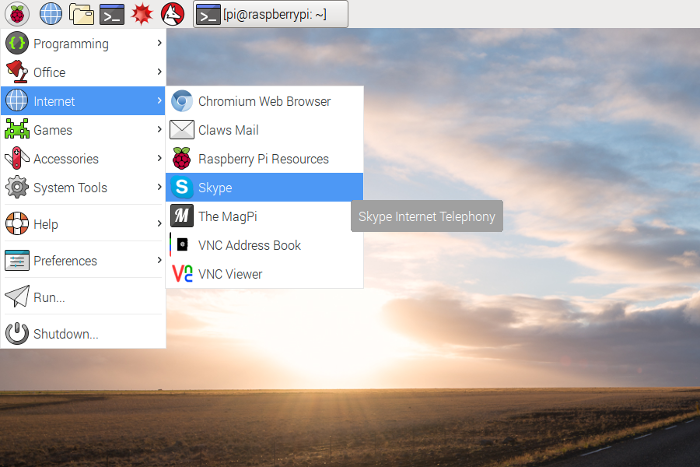
\includegraphics[scale=0.35]{img/skype.png} 
    \end{center}
\end{minipage}
\\

%%%%%%%%%%%%%%%%%%%%%%%%%%%%%%%%%%%%%%%%%%%%%%%%%%%%%%%%%%%%%%%%%%%%%%%%%%
\textbf{Skype Installieren}
\begin{verbatim}
7.Laden Sie Skype für Debian herunter:
  wget http://download.skype.com/linux/skype-debian_4.3.0.37-1_i386.deb
8.Installieren Skype:
  sudo dpkg -i skype-debian_4.3.0.37-1_i386.deb; sudo apt-get install -f
  sudo sed -i 's/4\.3\.0\.37/8\.3\.0\.37/' /usr/bin/skype 
\end{verbatim}
%%%%%%%%%%%%%%%%%%%%%%%%%%%%%%%%%%%%%%%%%%%%%%%%%%%%%%%%%%%%%%%%%%%%%%%%%%
Skype ausführen und überprüfen Sie, ob Skype-Soundgeräte den PulseAudio-Server verwenden:\\

\begin{minipage}{\textwidth}
    \begin{center}        
        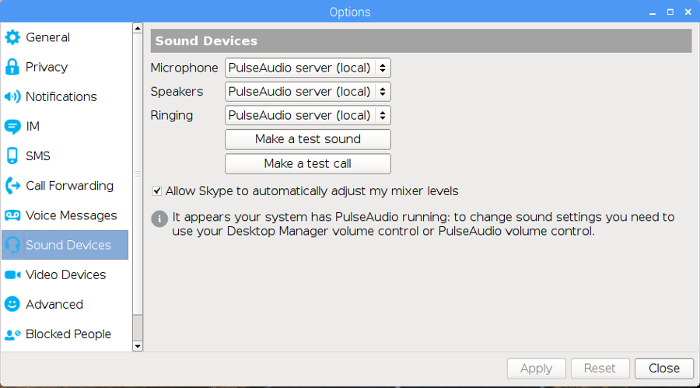
\includegraphics[scale=0.4]{img/skype-option.png} 
    \end{center}
\end{minipage}
\end{comment}
%%%%%%%%%%%%%%%%%%%%%%%%%%%%%%%%%%%%%%%%%%%%%%%%%%%%%%%%%%%%%%%%%%%%%%%%%%

\section{Gstreamer} \label{RefGstreamer}

%%%%%%%%%%%%%%%%%%%%%%%%%%%%%%%%%%%%%%%%%%%%%%%%%%%%%%%%%%%%%%%%%%%%%%%%%%
\subsection{Installation}
Mittels Paketmanager APT (Debian/Ubuntu), yum (Fedora/Centos) or homebrew (Mac) 
fehlende Pakete installieren, am Beispiel Ubuntu (Rapian Debian):
\begin{verbatim}
  sudo apt update 
  sudo apt install libgstreamer1.0-0 gstreamer1.0-plugins-base \
    gstreamer1.0-plugins-good gstreamer1.0-plugins-bad \
    gstreamer1.0-plugins-ugly gstreamer1.0-libav gstreamer1.0-doc \
    gstreamer1.0-tools
  sudo apt install libgstreamer1.0-dev
\end{verbatim}

%%%%%%%%%%%%%%%%%%%%%%%%%%%%%%%%%%%%%%%%%%%%%%%%%%%%%%%%%%%%%%%%%%%%%%%%%%
\textbf{I/O Elemente}
Ein Gstreamer Befehl ist aus einer Kette von Plugins aufgebaut. Die Verkettung der Befehle startet mit ein oder mehreren \textbf{src} Plugins und endet mit einem oder mehreren \textbf{sink} Plugins. Es folgt eine List mit src und sink Plugins.\\

\textbf{Beschreibung der verwendeten Eingangs oder SRC-Elemente}
\begin{itemize}
\item v4l2src – stream from a camera device on a linux system, e.g. device=/dev/video0;
\item audiotestsrc – used to do test streams with audio;
\item videotestsrc – used to do test streams with video, you may specify a pattern=<num>;
\item fakesrc – another option for testing by feeding in an empty stream;
\item filesrc – stream from a file, specifiy location=<filepath>;
\item ximagesrc – capture screen.
\end{itemize}

\textbf{Ausgabe oder SINK Elemente}
\begin{itemize}
\item filesink – save stream to a file, specify location=<filepath>;
\item  autoaudiosink – play audio on an automatically detected device;
\item  autovideosink – play video on an automatically detected display utility and device;
\item  fakesink – do not play stream, just finish;
\item  udpsink – stream result over UDP, specify host=<IP of the target server> and port=<number>;
\item rtmpsink – stream result over RTMP, specify host=<IP of the target server> and port=<number>.
\end{itemize}

\textbf{Kodierungselemente}\\
Die gstreamer Bibliothek umfasst Elemente um Streams zu komprimieren. Sie sind mit dem Kürzel 'enc' versehen, z.B. vorbis\textbf{enc}. Die Elemente zum Dekodieren eines Datenstroms verwenden dann das Kürzel 'dec' um die Daten zu dekomprimieren, z.B. vorbis\textbf{dec}.\\

\textbf{Audio}
\begin{itemize}
\item mp3 – lamemp3enc, avenc\_mp3 | mad, mpg123audiodec, avdec\_mp3; 
\item aac – voaccenc, faac, avenc\_aac | faad, aacparse, avdec\_aac;
\item vorbis – vorbisenc | vorbisdec, vorbisparse;
\item opus – opusenc, avenc\_opus | opusdec, avdec\_opus.
\end{itemize}

\textbf{Video}
\begin{itemize}
\item h.264 – x264enc, avh264\_enc |  h264parse, mpeg4videoparse, avdec\_h264;
\item mpeg2 -mpeg2enc, avenc\_mpeg2video | mpeg2dec, avdec\_mpeg2video;
\item jpeg2000 – no inter-frame coding, low latency; avenc\_jpeg2000 | avdec\_jpeg2000;
\item vp8 – vp8enc, avenc\_vp8 | vp8dec, avdec\_vp8;
\item vp9 – vp9enc, avenc\_vp9 | vp9dec, avdec\_vp9;
\item theora -theoraenc | theoradec, theoraparse.
\end{itemize}

%%%%%%%%%%%%%%%%%%%%%%%%%%%%%%%%%%%%%%%%%%%%%%%%%%%%%%%%%%%%%%%%%%%%%%%%%%

\textbf{Weitere Bestandteile der Pipeline}
\begin{itemize}
\item \textbf{Payers/Depayers} – Diese Elemente bereiten die (payload) Datapakete vor und holen die Daten nach dem Transport durchs Netzwerk wieder heraus. E.g.: rptvp8pay/rtpvp8depay, \\ rtph264/rtph264depay
\item \textbf{Konvertierer} – Diese Elemente können verwendet werden, um Manipulationen, wie z.B. Rotation, Farbraumtransformation, Skalierung auszuführen.
E.g.: audioconvert, audioresample, videoconvert, videoscale.
\end{itemize}
\color{black}
%%%%%%%%%%%%%%%%%%%%%%%%%%%%%%%%%%%%%%%%%%%%%%%%%%%%%%%%%%%
\subsection{Gstreamer Tests für Video \& Audio}

\textbf{Synthetische Quellen}

Video Test Source zum Display
\begin{verbatim}
Testbild:
  gst-launch-1.0 videotestsrc pattern=1 ! videoconvert ! autovideosink
Webcam oder intergrierte Kamera: 
  gst-launch-1.0 autovideosrc device=/dev/video0 ! autovideosink
\end{verbatim}

Audio Test Source zum Lautsprecher
\begin{verbatim}
  gst-launch-1.0 audiotestsrc ! audioconvert ! autoaudiosink
\end{verbatim}

Audio Test Quelle zu Fake Sink, aber trotzdem vollständige Pipeline
\begin{verbatim}
  gst-launch-1.0 audiotestsrc ! audioconvert ! fakesink
\end{verbatim}

Video Test Broadcast über TCP/HTTP
\begin{verbatim}
Sender
  gst-launch-1.0 videotestsrc horizontal-speed=5  ! vp8enc ! gdppay ! \
    tcpserversink host=127.0.0.1 port=5200
Empfänger
  gst-launch-1.0 -v tcpclientsrc port=5200 ! gdpdepay ! vp8dec ! \
    videoconvert ! autovideosink
\end{verbatim}

\textbf{Video Broadcast über RTP (via UDP) von der Webcam}
\begin{verbatim}
Sender
  gst-launch-1.0 v4l2src ! videoconvert ! video/x-raw, width=640,height=480 ! \
    omxh264enc ! rtph264pay pt=96 config-interval=1 ! \
    udpsink host=192.168.2.106 port =8554
Empfänger
  gst-launch-1.0 udpsrc port=8554 caps="application/x-rtp,media=video,\
    clockrate=90000,payload=96,encoding-name=H264" ! \
    rtph264depay ! avdec_h264 ! autovideosink
\end{verbatim}

\textbf{Video mit synthetischem Audio}
\begin{verbatim}
Sender:
  gst-launch-1.0 -v audiotestsrc ! audioconvert ! \
    audio/x-raw,channels=1,depth=16,width=16,rate=44100 ! rtpL16pay pt=97 ! \
    udpsink host=192.168.178.29 port=5001 v4l2src ! videoconvert ! \
    video/x-raw, width=640,height=480 ! omxh264enc ! \
    rtph264pay pt=96 config-interval=1 ! \
    udpsink host=192.168.178.29 port=5000
Empfänger
  gst-launch-1.0 udpsrc port=5001 ! application/x-rtp, clock-rate=44100, payload=97 ! 
    rtpL16depay ! audioconvert ! alsasink sync=false udpsrc port=5000 
    caps="application/x-rtp,media=video,payload=96,encoding-name=H264" ! rtph264depay !     
    avdec_h264 ! autovideosink
\end{verbatim}

\subsection{Kamera \& Mikrofon Streaming}
Erster Kamera Test:
\begin{verbatim}
  gst-launch-1.0 v4l2src ! xvimagesink
  gst-launch-1.0 v4l2src ! jpegdec ! xvimagesink
\end{verbatim}

\textbf{Video und Audio einer Webcam über RTP (in UDP Paketen)}
\begin{verbatim}
Sender
  gst-launch-1.0 -v alsasrc device=plughw:CARD=StudioTM,DEV=0 ! \
    audioconvert ! audio/x-raw,channels=1,depth=16,width=16,rate=44100 ! \
    rtpL16pay pt=97 ! udpsink host=192.168.178.29 port=5001 v4l2src ! \
    videoconvert ! video/x-raw, width=640,height=480 ! omxh264enc ! \
    rtph264pay pt=96 config-interval=1 ! udpsink host=192.168.178.29 port=5000
Empfänger
  gst-launch-1.0 udpsrc port=5001 ! application/x-rtp, clock-rate=44100,\
    payload=97 ! rtpL16depay ! audioconvert ! alsasink sync=false udpsrc \
    port=5000 caps="application/x-rtp,media=video,payload=96,encoding-name=H264" ! \
    rtph264depay ! avdec_h264 ! autovideosink
\end{verbatim}

\textbf{Raspi WebCam C920 Video/Audio an Webserver via RTP (UDP)}
\begin{verbatim}
Sender
  gst-launch-1.0 -v alsasrc device=plughw:1,0 ! audioconvert \
    ! audio/x-raw,channels=1,depth=16,width=16,rate=44100 \
    ! rtpL16pay pt=97 ! udpsink host=85.214.211.169 port=5001 v4l2src \
    ! videoconvert ! video/x-raw, width=640,height=480 ! omxh264enc \
    ! rtph264pay pt=96 config-interval=1 ! udpsink host=85.214.211.169 port=5000
\end{verbatim}

%%%%%%%%%%%%%%%%%%%%%%%%%%%%%%%%%%%%%%%%%%%%%%%%%%%%%%%%%%%%%%%%%%%%%%%%%%
\section{Janus-Gateway} \label{RefJanus}
Janus ist ein Server, der WebRTC Medien Kommunikation mit einem Browser unterstützt und json Nachrichten versendet. Zusätzlich können auch RTP/RTCP und Nachrichten zwischen Browsern und serverseitigen Programmen ausgetauscht werden. Plugins ermöglichen z.B. auch den Empfang von Streams im RTP/UDP Format versendet von Gstreamer. 

\subsection{Installation von Janus}
\begin{verbatim}
sudo apt install slibmicrohttpd-dev libjansson-dev libnice-dev \
	libssl-dev libsrtp-dev libsofia-sip-ua-dev libglib2.0-dev \
	libopus-dev libogg-dev libcurl4-openssl-dev liblua5.3-dev \
	pkg-config gengetopt libtool automake

git clone https://github.com/meetecho/janus-gateway.git
cd janus-gateway
sh autogen.sh

./configure --prefix=/opt/janus

sudo make 
sudo make install 
make configs

wenn ein libsrtp Fehler angezeigt wird libsrtp aus dem Quelen bauen:

wget https://github.com/cisco/libsrtp/archive/v2.0.0.tar.gz
tar xfv v2.0.0.tar.gz
cd libsrtp-2.0.0
./configure --prefix=/usr --enable-openssl
make shared_library && sudo make install
\end{verbatim}

%%%%%%%%%%%%%%%%%%%%%%%%%%%%%%%%%%%%%%%%%%%%%%%%%%%%%%%%%%%%%%%%%%%%%%%%%%%%%
\subsection{Konfiguration}
Zum Streaming via gstreamer RTP muss noch die cfg Datei angepasst werden.\\
Alle cfg Dateien liegen in: /opt/janus/etc/janus\\

In Datei: janus.transport.http.cfg
\begin{verbatim}
[general]
http = yes
ip = ...server-addr-ip-hostname
[admin]
admin_http = yes
\end{verbatim}

janus.plugin.streaming.cfg
\begin{verbatim}
[gst-rpwc]
type = rtp 
id = 1 
description = RPWC H264 test streaming 
audio = yes 
audioport = 8005 
audiopt = 10 
audiortpmap = opus/48000/2 
video = yes 
videoport = 8004 
videopt = 96 
videortpmap = H264/90000 
videofmtp = profile-level-id=42e028\;packetization-mode=1 
\end{verbatim}

%%%%%%%%%%%%%%%%%%%%%%%%%%%%%%%%%%%%%%%%%%%%%%%%%%%%%%%%%%%%%%%%%%%%%%%%%%%%%
\subsection{nginx Webserver} \label{Refnginx}
Installation von nginx Webserver zum Webseiten Testen in lokalem Netzwerk\\
Frei nach: https://www.digitalocean.com/community/tutorials/how-to-install-nginx-on-ubuntu-16-04
\begin{verbatim}
  sudo apt-get update
  sudo apt-get install nginx
  sudo ufw app list
\end{verbatim}

You should get a listing of the application profiles:\\
Terminal Ausgabe
\begin{verbatim}
Available applications:
  Nginx Full
  Nginx HTTP
  Nginx HTTPS
  OpenSSH
\end{verbatim}

Es ist meistens nötig Traffic auf dem Port 80 zu erlauben.\\
Man kann es konfigurieren mittels:
\begin{verbatim}
  sudo ufw allow 'Nginx HTTP'
  sudo ufw status
  http://server_domain_or_IP
\end{verbatim}

nginx Beispiele von janus nach /usr/share/nginx/html/demos kopieren
\begin{verbatim}
  sudo cp -r /opt/janus/share/janus/demos /usr/share/nginx/html/
\end{verbatim}
Im Browser unter http://ip-server/demos
wird trotzdem nur die Platzhalter Webseite angezeigt.

Um auf die kopierten Janus Webseiten zuzugreifen, muss noch etwas in der nginx Konfiguration geändert werden: /etc/nginx/sites-available
\begin{verbatim}
 #root /var/www/html;
 root /usr/share/nginx/html;
\end{verbatim}
Nun können die  Janus Beispiel html Dateien geladen werden.\\
http://192.168.178.25/demos/\\

Der Admin Monitor ist nur nach Eingabe eine Passwort verfügbar...\\
Entweder das Passwort aus /opt/janus/etc/janus/janus.cfg verwenden \\
(admin\_secret = janusoverlord) oder einfach wie folgt anpassen:
\begin{verbatim}
/usr/share/nginx/html/demos/admin.js
line 14
var secret = "janusoverlord";
\end{verbatim}
Danach ist das Passwort schon voreingestellt und wird nicht mehr abgefragt.\\
Nun kann der Admin Bereich im Browser geöffnet werden:
\begin{verbatim}
http://ip-server/demos
\end{verbatim}

%%%%%%%%%%%%%%%%%%%%%%%%%%%%%%%%%%%%%%%%%%%%%%%%%%%%%%%%%%%%%%%%%%%%%%%%%%%%%
\subsection{gstreamer an janus} \label{RefGstrToJanus}
Gstreamer Kommandos, um vom Raspberry V/A an das Janus-Gateway zu streamen\\
Zwei verschiedene Webcams wurden gestetet. \\
(1) Webcam HD Pro: CARD=C920,DEV=0 \\
(2) Microsoft® LifeCam Studio(TM): Webcam CARD=StudioTM,DEV=0 \\
Webcam (2) unterstützt h264parse nicht. Die Pipeline wurde alterntiv mit 
omxh264enc ergänzt. 
\begin{verbatim}
Webcam HD Pro: CARD=C920,DEV=0
  gst-launch-1.0 -v v4l2src ! h264parse ! rtph264pay config-interval=1 pt=96 ! \
    udpsink host=192.168.178.25 port=8004 alsasrc device=plughw:1,0 ! \ 
    audioconvert ! audioresample ! opusenc ! rtpopuspay ! udpsink \ 
    host=192.168.178.25 port=8005
 
Microsoft® LifeCam Studio(TM): Webcam CARD=StudioTM,DEV=0
Mit Bildskalierung, aber langsames Streamig (häufige Aussetzer)
  gst-launch-1.0 v4l2src ! videoconvert ! video/x-raw, width=640,height=480 !\
    omxh264enc ! rtph264pay pt=96 config-interval=1 ! \ 
    udpsink host=192.168.178.29 port=8004 alsasrc device=plughw:1,0 ! \
    audioconvert ! audioresample ! opusenc ! rtpopuspay ! udpsink \
    host=192.168.178.29 port=8005 
   
Microsoft® LifeCam Studio(TM): Webcam CARD=StudioTM,DEV=0
Ohne Bildskalierung, trotzdem schnelleres Streaming
  gst-launch-1.0 v4l2src ! omxh264enc ! rtph264pay pt=96 config-interval=1 ! \ 
    udpsink host=192.168.178.25 port=8006 alsasrc device=plughw:1,0 ! \
    audioconvert ! audioresample ! opusenc ! rtpopuspay ! udpsink \
    host=192.168.178.25 port=8007 
\end{verbatim}

%%%%%%%%%%%%%%%%%%%%%%%%%%%%%%%%%%%%%%%%%%%%%%%%%%%%%%%%%%%%%%%%%%%%%%%%%%
\section{Hardware}

%%%%%%%%%%%%%%%%%%%%%%%%%%%%%%%%%%%%%%%%%%%%%%%%%%%%%%%%%%%%%%%%%%%%%%%%%%%%%%%%%
\subsection{Raspberry Pi 3B+} \label{RefRaspi}
\textbf{Login via ssh}\\
Passwort und Benutzername können bereits bei der OP-Installation gesetzt werden. IP-Adresse kann über ip addr show abgefragt werden. Bei häufigen Verbindungen wird empfohlen eine statische IP-Adresse zu vergeben.\\

Bitte zuerst überprüfen, ob der ssh.service läuft.
\begin{verbatim}
/etc/init.d/ssh status
\end{verbatim}
Sollte eine Fehlermeldung erscheinen bitte ssh-server installieren.
\begin{verbatim}
sudo opt install openssh-server
\end{verbatim}
Falls nicht gestartet, in der Raspberry Konfiguration aktivieren:
\begin{verbatim}
  sudo raspi-config
\end{verbatim}
Danach ist es möglich über ssh einzuloggen.
\begin{verbatim}
  ssh pi@192.168.1.3
  pwd: xxxxxxxxxx (pwd vom Provider)
\end{verbatim}

\textbf{Raspberry Touchscreen Anzeige per Software drehen}
Wenn das Raspberry 7\grqq{} Display ins Gehäuse eingebaut wird ist die 
Visualisierung des Desktops 180 Grad verdreht. Es müssen Bildschirmanzeige 
und Toucherkennung gedreht werden. Softwaretechnisch sind dies zwei verschiedene 
Dinge.\\

\textbf{RASPIAN OP}\\
Display \& Touchscreen können mit einem Befehl rotiert werden, 
bitte in /boot/config.txt eintragen:
\begin{verbatim}
  lcd_rotate=2
\end{verbatim}

\textbf{Andere OP}\\
Hier wird mittels des lcd\_display Befehls nur der Touchbildschirm  gedreht. Es kann xrandr verwendet werden, um zusätzlich die visuelle Darstellung um 180 Grad zu drehen. Display Infos \& drehen:
\begin{verbatim}
  xrandr -q
  xrandr --output HDMI-1 --rotate inverted
\end{verbatim}


%%%%%%%%%%%%%%%%%%%%%%%%%%%%%%%%%%%%%%%%%%%%%%%%%%%%%%%%%%%%%%%%%%%%%%%%%%%%%%%%%
\subsection{Strato Web Server} \label{RefStrato}
\textbf{Login via ssh}
\begin{verbatim}
  ssh -X root@85.214.211.169
  ssh -X root@85.214.211.169 -L 5901:localhost:5901
  pwd: xxxxxxxxxx (pwd vom Provider)
\end{verbatim}
\textbf{Remote Desktop}\\
tightvncserver: server\\
xtightvncviewer: viewer
\begin{verbatim}sudo apt install tightvncserver xtightvncviewer
  set xtightvnciewer pwd
\end{verbatim}

\textbf{Full Login}
\begin{verbatim}
  ssh -X root@85.214.211.169 -L 5901:localhost:5901
  ssh Passwort eingeben
\end{verbatim}
Start vncserver
\begin{verbatim}
  vncserver :1
  echo "$DISPLAY"
\end{verbatim}
in server ssh console
\begin{verbatim}
  xtightvncviewer 127.0.0.1:1
  vnc Passwort eingeben
  Sollte eine Fehlermeldung erscheinen, mit htop
  F3 (search) htop suchen 
  ESC
  F9 (kill)
  2 SIGINT oder 9 SIGKILL
  und vnc Server nochmal starten
\end{verbatim}
X Fenster sollte sich öffnen\\

Dateien auf Server übertragen:
\begin{verbatim}
  scp <source> <destination>
  To copy a file from B to A while logged into B:
  scp /path/to/file username@a:/path/to/destination
  To copy a file from B to A while logged into A:
  scp username@b:/path/to/file /path/to/destination
\end{verbatim}
Beispiele:
\begin{verbatim}
Herunterladen aus der ssh Konsole: logged in PC -> eigener PC
  scp local_file_logged_in_pc user@my_own_host:dir_of_new_file_location
z.B. Herunterladen auf eigenen PC:
  scp /home/pi/Software/test/output.avi ts@192.168.178.25:/home/ts/Documents/tmp/
Hochladen aus lokaler Konsole: PC -> remote PC (raspberry)
  scp path_to_my_local_file pi@pi_host:dir_on_remote_pc
\end{verbatim}


%%%%%%%%%%%%%%%%%%%%%%%%%%%%%%%%%%%%%%%%%%%%%%%%%%%%%%%%%%%%%%%%%%%%%%%%%%%%%%%%%
\subsection{Audio Lautsprecher} \label{RefLautsprecher}
Die richtige Zuordnung setzen, sonst gibt es nur Sound vom 
Abspielen bei Audiodateien, aber nicht im Browser. Bitte im 
Browser, z.B. mit YouTube. '1' steht für local audio jack über 
den der Lautsprecher angeschlossen ist:
\begin{verbatim}
  amixer cset numid=3 1
  amixer cset numid=2 1
  oder
  amixer -c 0 cset numid=3 1
\end{verbatim}

\textbf{Audio Tests}
\begin{verbatim}
  aplay /usr/share/scratch/Media/Sounds/Vocals/Singer1.wav
\end{verbatim}
Facebook Video Call: OK (schlechter Sound)\\
Musikvidoes auf YouTube: OK (guter Sound)\\

Kommandozeile, um alle Audiogeräte anzuzeigen:\\
pacmd list-sources

Listet alle *.ogg Audiodateien auf dem ubuntu Rechner auf:\\
pacmd list-samples\\
Lautsprechertest (abspielen):\\
mplayer /usr/share/sounds/ubuntu/stereo/button-pressed.ogg 

%%%%%%%%%%%%%%%%%%%%%%%%%%%%%%%%%%%%%%%%%%%%%%%%%%%%%%%%%%%%%%%%%%%%%%%%%%%%%%%%%%%%
\subsection{Mikrofon der Webcam}
Anzeigen, ob Webcam erkannt wurde.\\
pacmd list-sources\\ 

Audio Stream aufnehmen:
\begin{verbatim}
  arecord -D plughw:1,0 -f cd test.wav
\end{verbatim}
abspielen mit:
\begin{verbatim}
  aplay test.wav
\end{verbatim}

Falls Hardwarekennung unbekannt, zeige alle Geräte:
\begin{verbatim}
  arecord -L
\end{verbatim}
Interessant ist der letzte Eintrag plughw, diesen kann man direkt für
ffmpeg verwenden, z.B.:
\begin{verbatim}
  webcam: ...plughw:CARD=C920,DEV=0 ...
  usb-micro: arecord -D plughw:CARD=C920,DEV=0 -f cd test.wav
\end{verbatim}

Wenn beim Testen mit ffmpeg der Fehler: 
\textbf{Unknown input format: 'alsa'}\\ 
auftreten, muss ffmpeg aus den Quellen kompiliert werden, siehe 
Softwarekapitel oder\\ 
https://lb.raspberrypi.org/forums/viewtopic.php?t=205181



\section{Glossar}
Beschreibung der wichtigsten Abkürzungen, die in der Übung verwendet werden.\\

\textbf{Glossar}\\
\textbf{PS}	Processing System, z.B. PS memory \\
\textbf{PL} Programmable Logic, z.B. PL memory\\
\textbf{AXI} Advanced eXtensible Interface as protocol for Intellectual Property (IP) cores\\


\end{document}
